 \chapterhead{CHƯƠNG 2 $-$ GIAO THỨC TRONG VPN}
 \addcontentsline{toc}{chapter}{CHƯƠNG 2 $-$ GIAO THỨC TRONG VPN}

 Để bảo mật các dữ liệu trong hệ thống VPN, có một số giao thức phổ biến được áp dụng vào mô hình. Tuy nhiên, tuỳ theo từng lớp ứng dụng cụ thể mà mỗi giao thức đều có ưu và nhược điểm khác nhau khi triển khai vào mạng VPN.
    
 \section*{2.1 Giao thức PPTP}
 \addcontentsline{toc}{section}{2.1 Giao thức PPTP}
 \subsection*{2.1.1 Khái quát giao thức PPTP}
 \addcontentsline{toc}{subsection}{2.1.1 Khái quát giao thức PPTP}

 PPTP (Point-to-Point Tunneling Protocol) là một giải pháp độc quyền cung cấp khả năng bảo mật giữa Remote Client và Enterprise Server bằng việc tạo ra một VPN thông qua một IP trên cơ sở mạng trung gian. Được phát triển vào năm 1999 bởi một nhóm nhà cung cấp, thành lập bởi Microsoft, Ascend Communications (một phần của Nokia), 3Com và nhiều nhóm khác. PPTP không những tạo ra điều kiện dễ dàng cho việc bảo mật các giao dịch thông qua TCP/IP trong môi trường mạng chung, mà còn qua mạng riêng Intranet. 

 
 \begin{figure}[htbp]
    \centering
    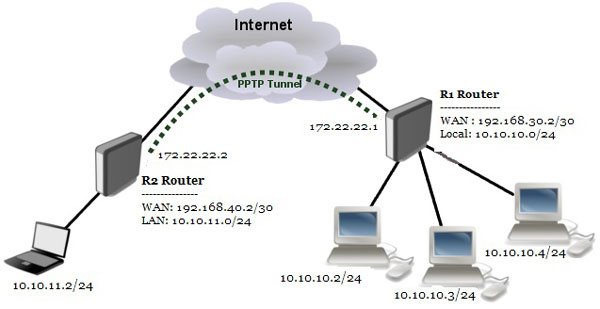
\includegraphics[width=0.7\linewidth]{img/pptp.png}
    \caption{Mô hình giao thức PPTP}
 \end{figure}
PPTP là một trong số nhiều kỹ thuật được sử dụng để thiết lập đường hầm cho những kết nối từ xa. Giao thức PPTP là một sự mở rộng của giao thức PPP (Point-to-Point) cơ bản cho nên giao thức PPTP không hỗ trợ những kết nối nhiều điểm liên tục mà nó chỉ hỗ trợ kết nối điểm tới điểm.

PPTP chỉ hỗ trợ IP, IPX, Net BEUI, PPTP không làm thay đổi PPP mà nó chỉ là giải pháp mới, một cách tạo đường hầm trong việc chuyên chở giao thông PPP.
    \begin{figure}[htbp]
        \centering
        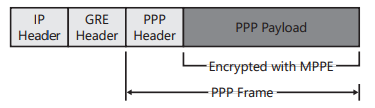
\includegraphics[width=0.7\linewidth]{img/packetPPTP.png}
        \caption{Cấu trúc gói tin của PPTP}
    \end{figure}
 \subsection*{2.1.2 Nguyên tắc hoạt động}
 \addcontentsline{toc}{subsection}{2.1.2 Nguyên tắc hoạt động}
 
   PPTP làm việc ở lớp liên kết dữ liệu trong mô hình OSI, bao gồm các phương thức đóng gói, tách gói tin IP và truyền gói tin từ máy này sang máy khác.
   
    Khi sử dụng PPTP, các gói dữ liệu IP được "đóng gói" bên trong các gói GRE và truyền đi qua một kết nối TCP trên cổng 1723. Để đảm bảo tính bảo mật, dữ liệu bên trong các gói PPP có thể được mã hóa và nén trước khi truyền đi. PPTP sử dụng giao thức PPP để quản lý các kết nối và truyền tải dữ liệu, bao gồm cả việc xác thực người dùng và quản lý lỗi.

    Cơ chế xác thực người dùng thường được cung cấp bới ISP, việc xác thực trong quá trình thiết lập kết nối PPTP sử dụng cơ chế xác thực của PPP. 
    
    Một số cơ chế được sử dụng:
    \begin{itemize}[left=2.5cm]
        \item Xác thực mở rộng EAP
        \item Xác thực có thử thách bắt tay CHAP
        \item Xác thực mật khẩu PAP
    \end{itemize}

    EAP tăng cường bảo mật cho mạng bằng cách cung cấp nhiều phương thức xác thực mạnh mẽ. Giao thức PAP là một cơ chế xác thực hoạt động dựa trên nguyên tắc mật khẩu được gửi qua các kết nối và không bảo mật. CHAP là một giao thức xác thực mạnh hơn, sử dụng phương pháp bắt tay ba chiều để hoạt động và ngăn chặn các cuộc tấn công bằng cách sử dụng các giá trị bí mật duy nhất và không thể đoán được.
    
    Khi PPP được thiết lập kết nối, PPTP sử dụng quy luật đóng gói của PPP để đóng gói các gói truyền thông trong đường hầm. PPTP định nghĩa hai loại gói tin là điều khiển và dữ liệu, sau đó chúng được gán vào các kênh riêng biệt. PPTP tách các kênh điều khiển và kênh dữ liệu thành những luồng điều khiển với giao thức điều khiển truyền dữ liệu TCP và luồng dữ liệu với giao thức IP.

    Các gói điều khiển PPTP đóng vai trò như những "tin nhắn" được trao đổi liên tục giữa máy khách và máy chủ để quản lý kết nối. Chúng chứa đựng các thông tin như trạng thái kết nối, thông tin cấu hình và thông tin xác thực người dùng. Nhờ đó, máy chủ có thể xác minh danh tính của người dùng, cấp quyền truy cập và đảm bảo rằng kết nối luôn được duy trì ổn định. Các loại gói điều khiển phổ biến bao gồm gói yêu cầu kết nối, gói xác nhận và gói giữ sống.

    Kênh điều khiển PPTP được sử dụng để thiết lập, quản lý và duy trì đường hầm VPN. Qua kênh này, máy khách và máy chủ trao đổi các gói tin điều khiển để xác thực danh tính, cấu hình kết nối và đảm bảo chất lượng dịch vụ. Các gói tin này được mã hóa bằng các giao thức như MPPE để bảo vệ thông tin khỏi bị nghe lén. Nhờ kênh điều khiển, người dùng có thể truy cập an toàn vào mạng nội bộ từ xa.
    \subsection*{2.1.3 Ưu điểm của PPTP}
    \addcontentsline{toc}{subsection}{2.1.3 Ưu điểm của PPTP}
    \begin{itemize}
        \item \textit{Dễ dàng thiết lập:}
        
        PPTP được đánh giá cao bởi tính dễ sử dụng. Giao thức này đã được tích hợp sẵn vào hầu hết các hệ điều hành phổ biến, từ Windows, macOS cho đến các bản phân phối Linux. Điều này giúp người dùng tiết kiệm đáng kể thời gian và công sức trong quá trình cài đặt và cấu hình. Hơn nữa, giao diện người dùng trực quan của các hệ điều hành hiện đại càng đơn giản hóa việc thiết lập kết nối VPN, giúp người dùng không chuyên cũng có thể dễ dàng thực hiện.
        \item \textit{Tốc độ kết nối cao:}

        Nhờ thuật toán mã hóa tương đối đơn giản, PPTP giảm thiểu đáng kể lượng tính toán cần thiết, từ đó tăng tốc độ truyền dữ liệu. Điều này đặc biệt hữu ích cho các ứng dụng đòi hỏi băng thông lớn như truyền tải video, chơi game trực tuyến hoặc làm việc từ xa.

        \item \textit{Độ tương thích rộng rãi:}

        PPTP được hỗ trợ bởi đa dạng các hệ điều hành và thiết bị mạng, từ máy tính để bàn, máy tính xách tay đến điện thoại di động và các thiết bị IoT. Tính tương thích cao này giúp người dùng dễ dàng thiết lập kết nối VPN trên nhiều thiết bị khác nhau mà không gặp quá nhiều khó khăn.
    \end{itemize}
    \subsection*{2.1.4 Nhược điểm của PPTP}
    \addcontentsline{toc}{subsection}{2.1.4 Nhược điểm của PPTP}

    \begin{itemize}
        \item \textit{Mã hoá yếu:}

        PPTP sử dụng các thuật toán mã hóa lỗi thời như RSA và RC4, vốn đã được chứng minh là không đủ mạnh để bảo vệ dữ liệu trước các cuộc tấn công hiện đại, độ dài khóa 128-bit của PPTP cũng không còn đảm bảo an toàn. Hơn nữa, giao thức này thiếu các tính năng bảo mật nâng cao như PFS, khiến nó dễ bị khai thác nếu khóa chính bị xâm phạm.

         \item \textit{Hiệu suất kém:}

         PPTP thường gặp phải các vấn đề về hiệu suất khi kết nối qua các mạng không ổn định hoặc có độ trễ cao. Giao thức này không được tối ưu hóa để hoạt động tốt trong các điều kiện mạng khắc nghiệt, dẫn đến tình trạng gián đoạn kết nối, tăng ping và làm giảm tốc độ truyền dữ liệu.
         \item \textit{Dễ bị tấn công:} 

         PPTP đã được phát hiện nhiều lỗ hổng bảo mật nghiêm trọng, khiến nó trở thành mục tiêu dễ bị tấn công của tin tặc. Các cuộc tấn công như man-in-the-middle có thể dễ dàng thực hiện trên các kết nối PPTP, cho phép kẻ tấn công đánh cắp dữ liệu một cách dễ dàng.
         
         \item \textit{Không phù hợp với nhu cầu hiện đại:}

         PPTP không đáp ứng được các yêu cầu bảo mật ngày càng cao của người dùng và doanh nghiệp. Giao thức này không hỗ trợ các tiêu chuẩn bảo mật hiện đại và thiếu các tính năng linh hoạt cần thiết để bảo vệ dữ liệu trong môi trường mạng phức tạp.
    \end{itemize}
 \section*{2.2 Giao thức L2TP/IPSec }
 \addcontentsline{toc}{section}{2.2 Giao thức L2TP/IPSec }
  \subsection*{2.2.1 Khái quát giao thức L2TP/IPSec}
 \addcontentsline{toc}{subsection}{2.2.1 Khái quát giao thức L2TP/IPSec}

 
 L2TP (Layer 2 Tunneling Protocol) là một giao thức tunneling được thiết kế để hỗ trợ các kết nối VPN. Thật thú vị, L2TP thường được ISP sử dụng để cho phép hoạt động VPN. L2TP được ra mắt lần đầu tiên vào năm 1999. Nó được thiết kế như một sự kế thừa của PPTP, do cả Microsoft và Cisco phát triển. Giao thức này sử dụng các tính năng khác nhau từ giao thức PPTP của Microsoft và L2F (Layer 2 Forwarding) của Cisco, sau đó cải thiện chúng.

  \begin{figure}[htbp]
        \centering
        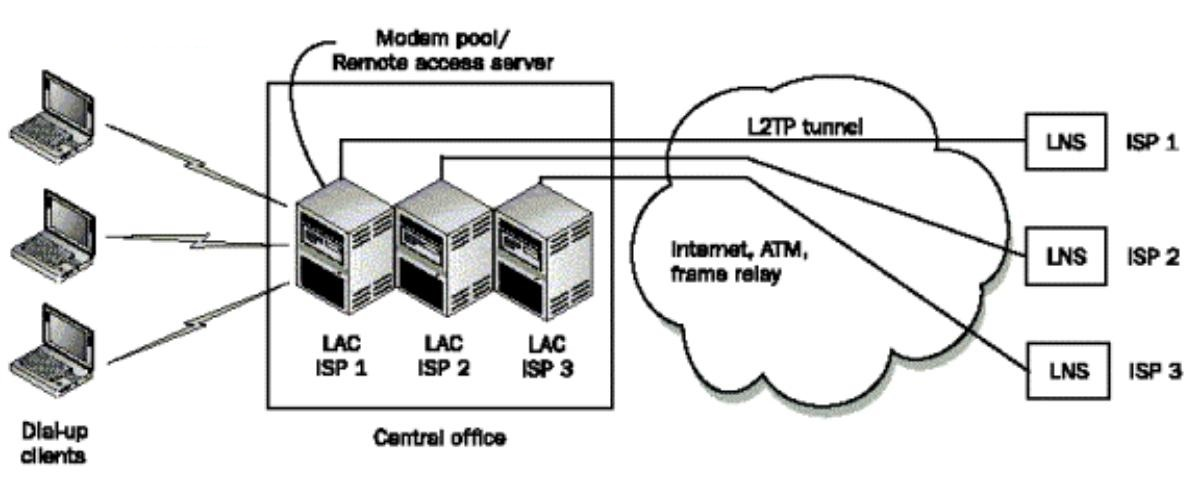
\includegraphics[width=0.8\linewidth]{img/l2tp.jpeg}
        \caption{Mô hình giao thức L2TP}
    \end{figure}

 IPSec (Internet Protocol Security) là một bộ giao thức bảo mật được thiết kế để mã hóa và xác thực dữ liệu trong quá trình truyền thông tin, điểu khiển truy nhập, bảo vệ chống phát lại và bảo mật. IPSec được sử dụng như một chức năng xác thực và được gọi là Authentication Hearder (AH). Được dùng trong việc mã hoá, kết hợp chức năng gọi là Encapsulating Security Payload (ESP).

 L2TP thường được ghép nối với IPsec vì bản thân nó không mã hóa dữ liệu. Sự kết hợp của L2TP và IPsec đảm bảo tính bảo mật, toàn vẹn và xác thực của các gói dữ liệu được truyền qua đường hầm VPN. Cấu trúc gói tin thể hiện IPSec thực hiện cả hai việc là mã hóa và ký số để bảo vệ cho gói dữ liệu L2TP được đóng gói trong header của nó.
 
 \begin{figure}[htbp]
        \centering
        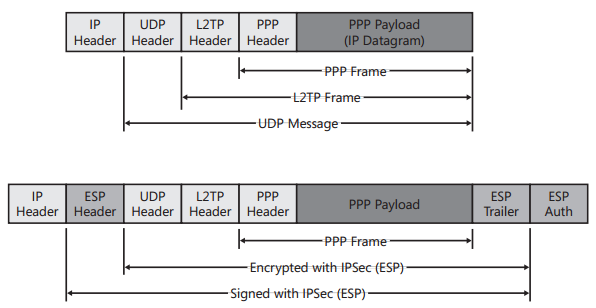
\includegraphics[width=0.7\linewidth]{img/l2tp-packet-structure.png}
        \caption{Cấu trúc gói tin của L2TP}
    \end{figure}

 \subsection*{2.2.2 Nguyên tắc hoạt động}
 \addcontentsline{toc}{subsection}{2.2.2 Nguyên tắc hoạt động}

 Giai đoạn đầu tiên trong quy trình hoạt động của L2TP/IPSec là việc tạo một kết nối đường hầm giữa thiết bị khách và máy chủ VPN thông qua giao thức L2TP. Dữ liệu trong đường hầm đó sẽ được đóng gói để truyền tải giữa hai điểm. Trong quá trình này, thiết bị khách gửi yêu cầu kết nối đến máy chủ VPN, và máy chủ sẽ xác nhận để hoàn thành việc thiết lập đường hầm. Đặc điểm quan trọng của giai đoạn này là L2TP chỉ đảm nhận việc tạo đường hầm và không thực hiện mã hóa hoặc bảo mật dữ liệu, khiến nó cần sự hỗ trợ của giao thức bảo mật IPSec trong các giai đoạn tiếp theo.

 Sau khi đường hầm L2TP được thiết lập, IPSec sẽ được kết hợp để cung cấp tính năng bảo mật. Trong giai đoạn này, IPSec sử dụng giao thức IKE để thương lượng các tham số bảo mật giữa thiết bị khách và máy chủ. Hai bên sẽ đồng thuận về các thuật toán mã hóa và phương pháp xác thực, chẳng hạn như AES hoặc 3DES, để đảm bảo kết nối an toàn. Quá trình này được gọi là thiết lập SA. Khi giai đoạn này hoàn tất, tất cả dữ liệu truyền qua đường hầm L2TP sẽ được mã hóa và bảo vệ bởi IPSec, tạo nền tảng cho một kết nối VPN an toàn.

 Để đảm bảo tính toàn vẹn và bảo mật của dữ liệu, L2TP/IPSec sẽ thực hiện quá trình xác thực và mã hóa. Thiết bị khách và máy chủ VPN sẽ tiến hành xác thực lẫn nhau thông qua các phương pháp như khóa chia sẻ trước hoặc chứng chỉ số. Sau khi xác thực, dữ liệu trong đường hầm sẽ được mã hóa bằng các thuật toán mạnh như AES-256, đảm bảo rằng thông tin không thể bị đọc lén hoặc thay đổi trong quá trình truyền tải. Đồng thời, các cơ chế kiểm tra toàn vẹn (Integrity Check) sẽ được thực hiện để đảm bảo rằng mọi gói dữ liệu được truyền tải đều nguyên vẹn và không bị sửa đổi.

 Khi việc xác thực và mã hóa hoàn tất, dữ liệu sẽ được truyền qua đường hầm bảo mật do L2TP/IPSec tạo ra. Nhờ lớp mã hóa của IPSec, dữ liệu được bảo vệ khỏi các cuộc tấn công như nghe lén hoặc chỉnh sửa trái phép. Đồng thời, cơ chế xác thực của IPSec đảm bảo rằng chỉ các gói dữ liệu hợp lệ mới được xử lý. Quá trình truyền tải này mang lại sự an toàn cao cho thông tin, đồng thời đảm bảo rằng dữ liệu được gửi đến đúng đích mà không bị gián đoạn.
 \subsection*{2.2.3 Ưu điểm của L2TP/IPSec}
 \addcontentsline{toc}{subsection}{2.1.3 Ưu điểm của L2TP/IPSec}

   \begin{itemize}
        \item \textit{Bảo mật cao:}
        
        L2TP khi được kết hợp với IPSec mang lại một cấp độ bảo mật vượt trội nhờ cơ chế mã hóa và xác thực mạnh mẽ. IPSec cung cấp các thuật toán mã hóa tiên tiến như AES-256, đảm bảo rằng dữ liệu được bảo vệ toàn diện khỏi các cuộc tấn công nghe lén và sửa đổi dữ liệu trái phép. Ngoài ra, giao thức này còn hỗ trợ cơ chế kiểm tra tính toàn vẹn dữ liệu thông qua các hàm băm như HMAC, giúp loại bỏ hoàn toàn nguy cơ dữ liệu bị thay đổi trong quá trình truyền tải.
        \item \textit{Thân thiện với người dùng:}

        Giao thức L2TP rất dễ dàng để cấu hình và sử dụng, đặc biệt trên các hệ điều hành phổ biến như Windows, macOS, iOS và Android, được hỗ trợ mặc định mà không cần cài đặt phần mềm bổ sung. Các công cụ quản lý VPN tích hợp sẵn thường cung cấp giao diện thân thiện, giúp người dùng thiết lập kết nối nhanh chóng chỉ với một vài bước cơ bản.

        \item \textit{Linh hoạt:}

        L2TP là giao thức đa năng, có khả năng hoạt động trên nhiều nền tảng khác nhau và hỗ trợ các giao thức mạng khác nhau, bao gồm cả IPv4 và IPv6. Sự linh hoạt này giúp L2TP phù hợp với các môi trường mạng đa dạng, từ mạng doanh nghiệp phức tạp đến mạng gia đình đơn giản. 
    \end{itemize} 
 \subsection*{2.2.4 Nhược điểm của L2TP/IPSec}
 \addcontentsline{toc}{subsection}{2.1.4 Nhược điểm của L2TP/IPSec}

\begin{itemize}
        \item \textit{Hiệu suất kém:}
        
        L2TP/IPSec có hiệu suất thấp do dữ liệu phải mã hóa hai lần: một lần bởi L2TP và một lần bởi IPSec. Quá trình này tiêu tốn nhiều tài nguyên CPU, đặc biệt trên thiết bị yếu, và làm tăng kích thước gói tin, gây giảm tốc độ truyền tải, nhất là trên mạng có băng thông hạn chế.
        \item \textit{Firewall:}

        L2TP/IPSec dễ gặp vấn đề với tường lửa hoặc NAT. Giao thức ESP của IPSec thường bị chặn trong các môi trường mạng nghiêm ngặt hoặc không hỗ trợ tốt, dẫn đến lỗi kết nối VPN, đặc biệt trong các hệ thống có firewall phức tạp. Trong một số trường hợp, các mạng NAT không được cấu hình đúng cách cũng có thể khiến việc thiết lập kết nối VPN L2TP/IPSec thất bại, dẫn đến gián đoạn dịch vụ. Điều này khiến giao thức không phù hợp với các môi trường mạng có cấu hình phức tạp hoặc bị hạn chế mạnh mẽ.

        \item \textit{Cấu hình phức tạp:}

        Việc thiết lập L2TP/IPSec yêu cầu nhiều bước phức tạp, từ cấu hình IPSec song song với L2TP đến việc thiết lập khóa chia sẻ trước (PSK) hoặc chứng chỉ số. Điều này có thể gây khó khăn cho người dùng ít kinh nghiệm và mất nhiều thời gian để triển khai.
    \end{itemize} 

  \section*{2.3 Giao thức SSTP}
 \addcontentsline{toc}{section}{2.3 Giao thức SSTP }

 \subsection*{2.3.1 Khái quát giao thức SSTP}
 \addcontentsline{toc}{subsection}{2.2.1 Khái quát giao thức SSTP}
 SSTP (Secure Sockets Tunneling Protocol) là một loại giao thức VPN được phát triển bởi Microsoft. Do vậy, giao thức này được dùng phổ biến trong môi trường Windows hơn. Đây là giao thức phát triển nhằm thay thế cho giao thức PPTP kém an toàn và có sẵn trong Windows.

 SSTP được phát triển nhằm cho phép các VPN client kết nối tới VPN server mà cần xuyên qua các thành phần ngăn cản việc truyền nhận các gói tin PPTP, L2TP/IPSec như firewall, NAT, và Web proxy. SSTP làm được điều này bằng cách đóng gói các gói tin PPP trong một kênh HTTPS. SSTP sử dụng giao thức mã hóa SSL/TLS, có tính bảo mật cao, cho phép dữ liệu vượt trường lửa hiệu quả. SSTP sử dụng cùng một cổng với HTTPS, đảm bảo khả năng tương thích và dễ dàng truy cập qua Internet, cho phép truy cập từ xa an toàn và tin cậy, đồng thời bảo vệ quyền riêng tư và tính toàn vẹn dữ liệu.
\newpage
  \begin{figure}[htbp]
        \centering
        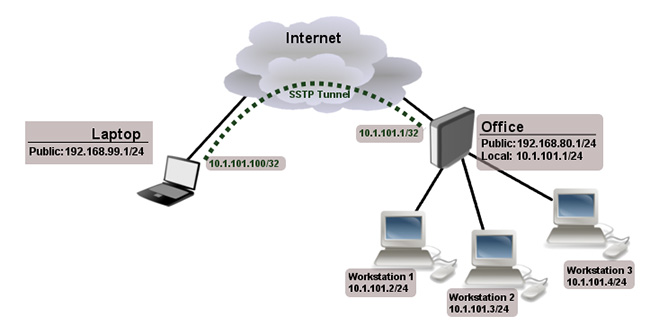
\includegraphics[width=0.8\linewidth]{img/sstp.jpeg}
        \caption{Mô hình giao thức SSTP}
    \end{figure}

 Gói dữ liệu PPP (gồm payload và header) được đóng gói trong một SSTP header rồi sau đó chúng được mã hóa bằng một phiên SSL. Để hoàn chỉnh gói tin, một TCP header và một IPv4 (hoặc IPv6) header được thêm vào. Nội dung của các header này (IP, port) có thể được chuyển đổi khi truyền qua các thiết bị firewall, NAT mà không làm thay đổi gói dữ liệu SSL được mã hóa.

     \begin{figure}[htbp]
        \centering
        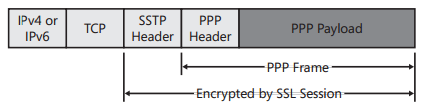
\includegraphics[width=0.8\linewidth]{img/sstp-packet-structure.png}
        \caption{Cấu trúc gói tin của SSTP}
    \end{figure}
  \subsection*{2.3.2 Nguyên tắc hoạt động}
  \addcontentsline{toc}{subsection}{2.2.2 Nguyên tắc hoạt động}

 Quy trình hoạt động của SSTP bắt đầu bằng việc thiết lập một kết nối bảo mật giữa thiết bị khách và máy chủ VPN thông qua giao thức HTTPS. Trong giai đoạn này, SSTP sử dụng SSL/TLS để tạo một kênh bảo mật, đảm bảo rằng kết nối được mã hóa ngay từ khi bắt đầu. Việc sử dụng HTTPS cho phép SSTP dễ dàng vượt qua các tường lửa và NAT, do hầu hết các mạng đều cho phép giao tiếp qua cổng 443. Đây là điểm đặc biệt giúp SSTP trở thành một lựa chọn đáng tin cậy trong các môi trường mạng hạn chế.

 Sau khi kết nối bảo mật được thiết lập, giai đoạn tiếp theo là xác thực. Trong bước này, cả thiết bị khách và máy chủ sẽ tiến hành xác minh danh tính của nhau. SSTP hỗ trợ các phương thức xác thực mạnh mẽ, chẳng hạn như sử dụng chứng chỉ số SSL/TLS và các giao thức xác thực người dùng như MS-CHAP v2. Điều này đảm bảo rằng chỉ các thiết bị và người dùng được ủy quyền mới có thể truy cập vào mạng VPN, tăng cường mức độ an toàn của kết nối.

 Khi việc xác thực hoàn tất, dữ liệu từ thiết bị khách sẽ được đóng gói trong đường hầm bảo mật do SSTP thiết lập. Trong giai đoạn này, các gói dữ liệu được mã hóa bằng SSL/TLS, đảm bảo rằng thông tin được bảo vệ khỏi các mối đe dọa như nghe lén hoặc chỉnh sửa dữ liệu trái phép. Việc mã hóa này không chỉ bảo vệ dữ liệu mà còn đảm bảo tính toàn vẹn, giúp gói tin đến đích mà không bị sửa đổi trong quá trình truyền tải.

 Giai đoạn cuối cùng là truyền dữ liệu qua giao thức HTTPS. Dữ liệu đã được mã hóa sẽ được gửi đi thông qua cổng 443, là cổng mặc định cho lưu lượng HTTPS. Điều này giúp SSTP dễ dàng vượt qua tường lửa và thiết bị NAT mà không cần cấu hình đặc biệt, vì lưu lượng HTTPS thường được phép trong mọi mạng. Quá trình này đảm bảo rằng dữ liệu được truyền tải an toàn, đáng tin cậy và không bị gián đoạn, ngay cả trong các môi trường mạng nghiêm ngặt.
 \subsection*{2.3.3 Ưu điểm của SSTP}
 \addcontentsline{toc}{subsection}{2.1.3 Ưu điểm của SSTP}

 \begin{itemize}
        \item \textit{Khả năng vượt qua Firewall:}
        
         SSTP sử dụng giao thức HTTPS qua cổng 443, vốn là cổng mặc định cho lưu lượng web an toàn, nên hầu hết các mạng đều cho phép kết nối qua cổng này. Điều này giúp SSTP hoạt động ổn định trong các môi trường mạng hạn chế hoặc bị kiểm soát nghiêm ngặt, nơi các giao thức VPN khác như L2TP hoặc PPTP có thể bị chặn.
        \item \textit{Bảo mật và xác thực mạnh mẽ:}

        SSTP sử dụng giao thức SSL/TLS để mã hóa và xác thực kết nối, mang lại một cấp độ bảo mật vượt trội. SSL/TLS sử dụng các thuật toán mã hóa mạnh như AES-256 và cơ chế kiểm tra toàn vẹn dữ liệu, đảm bảo rằng dữ liệu được bảo vệ toàn diện trước các mối đe dọa như nghe lén hoặc giả mạo. Đồng thời, SSTP hỗ trợ các phương pháp xác thực như MS-CHAP v2 và chứng chỉ số, tăng cường tính an toàn cho kết nối VPN.

        \item \textit{Tích hợp tốt với Windows:}

        SSTP được Microsoft phát triển và tích hợp sẵn trên các hệ điều hành Windows từ phiên bản Windows Vista SP1 trở đi. Người dùng Windows có thể dễ dàng thiết lập và sử dụng SSTP mà không cần cài đặt phần mềm bổ sung. Ngoài ra, SSTP cũng tích hợp tốt với các tính năng bảo mật khác của Windows, như Active Directory hoặc các chính sách mạng (Group Policy), giúp doanh nghiệp triển khai dễ dàng và hiệu quả hơn.
    \end{itemize} 
 
 \subsection*{2.3.4 Nhược điểm của SSTP}
 \addcontentsline{toc}{subsection}{2.1.4 Nhược điểm của SSTP}

 \begin{itemize}
        \item \textit{Tương thích bị hạn chế:}
        
         SSTP được Microsoft phát triển và chủ yếu hỗ trợ trên các hệ điều hành Windows. Mặc dù có thể cấu hình trên các hệ điều hành khác như Linux hoặc macOS, nhưng việc này không được hỗ trợ chính thức, gây ra nhiều khó khăn. Sự hạn chế trong tính tương thích khiến SSTP khó sử dụng trên các nền tảng phổ biến khác hoặc thiết bị di động không thuộc hệ sinh thái Windows.
        \item \textit{Tốc độ chậm:}

        SSTP sử dụng giao thức SSL/TLS để mã hóa, vốn tiêu tốn tài nguyên xử lý cao, đặc biệt khi sử dụng các thuật toán mã hóa mạnh như AES-256. Điều này làm giảm tốc độ truyền dữ liệu, đặc biệt trên các mạng có băng thông thấp hoặc thiết bị phần cứng yếu. 

        \item \textit{Khó thiết lập:}

        Mặc dù tích hợp tốt với Windows, việc thiết lập SSTP vẫn phức tạp hơn so với các giao thức VPN khác như PPTP. Người dùng cần phải cài đặt và cấu hình chứng chỉ số SSL/TLS trên máy chủ và thiết bị khách để đảm bảo kết nối an toàn. Quá trình này đòi hỏi kiến thức kỹ thuật và có thể gây khó khăn cho người dùng không chuyên.
    \end{itemize} 

    
 \section*{2.4 Giao thức IKEv2 }
 \addcontentsline{toc}{section}{2.4 Giao thức IKEv2 }

 \subsection*{2.4.1 Khái quát giao thức IKEv2}
 \addcontentsline{toc}{subsection}{2.4.1 Khái quát giao thức IKEv2} 

  IKEv2 (Internet Key Exchange Version 2) là một giao thức dựa theo công nghệ đường hầm IPsec, được phát triển bởi Cisco và Microsoft. Giao thức này hiện xuất hiện trên Windows 7 trở đi cũng như Linux và các nền tảng khác bao gồm cả  Blackberry. Nó có tác dụng tạo lại kết nối VPN một cách tự động khi kết nối bị ngắt tạm thời. IKEv2 có cái tên khác là Mobility and Multi-homing protocol là một chuẩn hóa giúp thay đổi mạng một cách dễ dàng. Ngoài ra, nó cũng khá hữu dụng với thiết bị Blackberry vì nó là số ít giao thức hỗ trợ cho nền tảng này.  Mặc dù hỗ trợ ít hệ điều hành hơn nếu so với  IPsec nhưng IKEv2 lại không thua kém về tính ổn định, bảo mật và hiệu suất.
 
  \subsection*{2.4.2 Nguyên tắc hoạt động}
 \addcontentsline{toc}{subsection}{2.4.2 Nguyên tắc hoạt động} 

 Giai đoạn đầu tiên của IKEv2 là quá trình thiết lập phiên ban đầu, được gọi là IKE\_SA\_INIT. Trong giai đoạn này, thiết bị khách và máy chủ trao đổi thông tin để thỏa thuận các tham số bảo mật như thuật toán mã hóa, hàm băm, và giao thức bảo mật IPSec. Đồng thời, cả hai bên sẽ thực hiện trao đổi khóa Diffie-Hellman để tạo ra khóa phiên chung, đảm bảo rằng kết nối ban đầu được bảo mật trước các mối đe dọa như nghe lén. Đây là bước quan trọng đặt nền móng cho việc truyền thông tin an toàn giữa hai bên.

 Sau khi thiết lập phiên ban đầu, giai đoạn thứ hai là IKE\_AUTH, nơi cả hai bên tiến hành xác thực lẫn nhau. Giai đoạn này sử dụng các cơ chế xác thực mạnh mẽ như khóa chia sẻ trước (PSK), chứng chỉ số, hoặc EAP để đảm bảo rằng cả thiết bị khách và máy chủ đều là những thực thể hợp lệ. Đồng thời, trong giai đoạn này, các tham số của kênh bảo mật IPSec (Child SA) cũng được thiết lập, cho phép truyền dữ liệu một cách an toàn sau khi xác thực thành công.

 Giai đoạn cuối cùng của IKEv2 tập trung vào việc duy trì và quản lý kết nối VPN. Giao thức IKEv2 hỗ trợ các tính năng như trao đổi lại khóa mã hóa (rekeying) để duy trì tính bảo mật trong suốt thời gian kết nối. Ngoài ra, nó còn có khả năng xử lý các sự cố như gián đoạn kết nối bằng cách sử dụng tính năng MOBIKE. Điều này giúp đảm bảo rằng kết nối VPN luôn ổn định và đáng tin cậy, ngay cả khi thiết bị di chuyển qua nhiều mạng hoặc thay đổi địa chỉ IP.
 
  \subsection*{2.4.3 Ưu điểm của IKEv2}
 \addcontentsline{toc}{subsection}{2.4.3 Ưu điểm của IKEv2} 

  \begin{itemize}
        \item \textit{Tốc độ và hiệu suất cao:}
        
         Một trong những ưu điểm lớn nhất của IKEv2 là khả năng tối ưu hóa tốc độ và hiệu suất. Giao thức này sử dụng ít bước trao đổi hơn so với các giao thức VPN khác như IKEv1, giúp giảm độ trễ và tăng tốc quá trình thiết lập kết nối. Điều này mang lại hiệu suất tốt hơn, đặc biệt trong các môi trường có băng thông hạn chế hoặc khi người dùng cần kết nối nhanh chóng.
        \item \textit{Ổn định và linh hoạt:}

        IKEv2 được thiết kế để duy trì kết nối ổn định trong suốt quá trình sử dụng. Với tính năng MOBIKE, IKEv2 có thể duy trì kết nối VPN ngay cả khi người dùng di chuyển qua các mạng khác nhau hoặc thay đổi địa chỉ IP, giúp đảm bảo kết nối không bị gián đoạn. Điều này rất hữu ích cho các thiết bị di động hoặc người dùng cần kết nối khi roaming qua các mạng Wi-Fi hoặc mạng di động.
        \item \textit{Bảo mật cao:}

        IKEv2 hỗ trợ các thuật toán mã hóa mạnh mẽ như AES và SHA, đảm bảo rằng dữ liệu được bảo vệ an toàn trong suốt quá trình truyền tải. Giao thức này cũng sử dụng các cơ chế xác thực mạnh như chứng chỉ số và khóa chia sẻ trước, giúp xác minh độ tin cậy của cả client và server trước khi thiết lập kết nối, tăng cường bảo mật cho mạng VPN.

        \item \textit{Khả năng tái kết nối tự động:}

        Một điểm mạnh khác của IKEv2 là khả năng tái kết nối tự động. Nếu kết nối VPN bị gián đoạn, IKEv2 có thể tự động khôi phục kết nối mà không cần người dùng can thiệp. Điều này giúp duy trì kết nối VPN ổn định và giảm thiểu các sự cố mạng, đặc biệt khi người dùng di chuyển hoặc khi có sự thay đổi trong mạng lưới.
    \end{itemize} 

 \subsection*{2.4.4 Nhược điểm của IKEv2}
 \addcontentsline{toc}{subsection}{2.4.4 Nhược điểm của IKEv2} 

  \begin{itemize}
        \item \textit{Hạn chế hỗ trợ thiết bị:}
        
         IKEv2 là một giao thức mạnh mẽ, nhưng nó không được hỗ trợ rộng rãi trên tất cả các thiết bị và hệ điều hành. Windows, MacOS và nhiều thiết bị di động hỗ trợ IKEv2, tuy nhiên ở các hệ điều hành khác, đặc biệt là các bản Linux hoặc các thiết bị không phải của Microsoft, có thể gặp khó khăn trong việc triển khai hoặc thiếu sự hỗ trợ chính thức cho giao thức này. Điều này hạn chế khả năng sử dụng IKEv2 trong các môi trường đa nền tảng hoặc trên các thiết bị không tương thích.
        \item \textit{Cấu hình phức tạp:}

        Việc thiết lập và cấu hình nó có thể phức tạp, đặc biệt đối với người dùng không có nhiều kinh nghiệm trong việc cấu hình VPN. Các tham số bảo mật như chứng chỉ số, khóa chia sẻ trước và cấu hình mạng yêu cầu sự hiểu biết kỹ thuật và có thể gây khó khăn trong quá trình triển khai. Điều này có thể làm tăng thời gian và chi phí triển khai, đặc biệt đối với các tổ chức nhỏ hoặc người dùng cá nhân.
       
        \item \textit{Khả năng bị chặn bởi Firewall:}

        Mặc dù IKEv2 có khả năng vượt qua một số rào cản tường lửa nhờ sử dụng các cổng mặc định, như cổng UDP 500 và 4500, nhưng nó vẫn có thể gặp khó khăn trong các môi trường mạng có tường lửa nghiêm ngặt hoặc không hỗ trợ các giao thức IPSec. Điều này có thể gây ra sự cố trong việc kết nối và yêu cầu cấu hình thêm để vượt qua các hạn chế của tường lửa hoặc NAT.
    \end{itemize} 
 
 \section*{2.5 Giao thức OpenVPN}
 \addcontentsline{toc}{section}{2.5 Giao thức OpenVPN}

 \subsection*{2.5.1 Khái quát giao thức OpenVPN}
 \addcontentsline{toc}{subsection}{2.5.1 Khái quát giao thức OpenVPN} 

OpenVPN được tạo ra vào năm 2001, là một giao thức mã nguồn mở được sử dụng rộng rãi để thiết lập kết nối VPN an toàn. Giao thức này hoạt động dựa trên các công nghệ mã hóa mạnh mẽ như SSL/TLS để đảm bảo tính bảo mật, riêng tư và toàn vẹn dữ liệu khi truyền qua các mạng không an toàn, bao gồm cả Internet. OpenVPN hỗ trợ nhiều nền tảng như Windows, macOS, Linux, iOS, Android và các thiết bị nhúng, làm cho nó trở thành một lựa chọn phổ biến trong cả môi trường cá nhân và doanh nghiệp.

OpenVPN có thể được sử dụng cho nhiều mục đích.

 - \textit{Như một giao thức:} Khi triển khai dưới dạng giao thức, nó cung cấp tốc độ tốt và bảo mật mạnh mẽ, có thể sử dụng cùng với mã hóa hàng đầu ngành. Đây cũng là một trong những giao thức phổ biến nhất được sử dụng cho cài đặt router.

 - \textit{Như một phần mềm:} Một số hệ thống có thể quá cũ để chạy ứng dụng VPN tốt, nhưng chúng có thể chạy được phần mềm OpenVPN. Hơn nữa, phần mềm OpenVPN là một cách tuyệt vời để vượt qua các hạn chế mạng nơi dịch vụ VPN bị chặn. Điều này có thể là mạng làm việc của bạn chặn tải xuống dịch vụ VPN hoặc tường lửa quốc gia như Tường Lửa Lớn của Trung Quốc chặn truy cập hoàn toàn các trang web VPN.
\subsection*{2.5.2 Nguyên tắc hoạt động}
 \addcontentsline{toc}{subsection}{2.5.2 Nguyên tắc hoạt động} 

OpenVPN hoạt động bằng cách thiết lập một kênh kết nối an toàn giữa máy khách và máy chủ thông qua các giao thức mã hóa mạnh như SSL/TLS. Khi máy khách gửi yêu cầu kết nối, máy chủ xác thực danh tính của máy khách bằng các phương pháp như chứng chỉ số, tên người dùng và mật khẩu, hoặc mã khóa chia sẻ.

Sau khi xác thực thành công, một kênh mã hóa được thiết lập để bảo vệ dữ liệu trong quá trình truyền tải. Dữ liệu từ máy khách được đóng gói vào các gói OpenVPN, mã hóa và gửi qua mạng. Máy chủ sau đó giải mã dữ liệu và định tuyến đến đích, đảm bảo tính bảo mật và toàn vẹn dữ liệu.

Ngoài ra, OpenVPN hỗ trợ nén dữ liệu để cải thiện hiệu suất, đồng thời sử dụng các thuật toán băm để kiểm tra tính toàn vẹn của dữ liệu, giúp phát hiện các thay đổi trái phép trong quá trình truyền tải.

\begin{figure}[htbp]
        \centering
        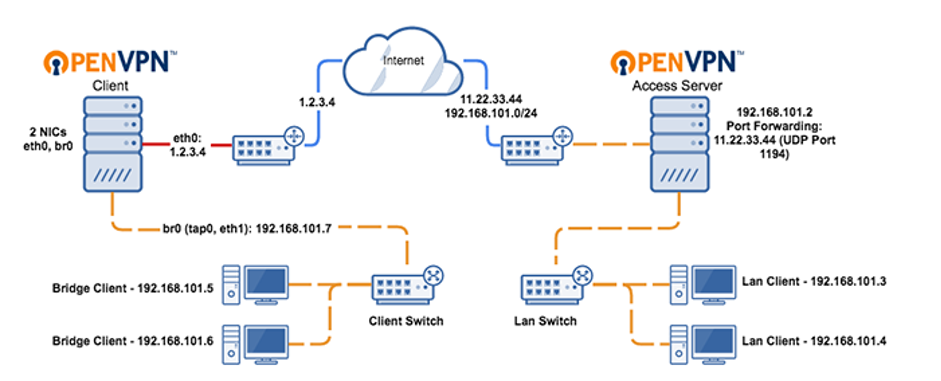
\includegraphics[width=0.8\linewidth]{img/openvpn.png}
        \caption{Cơ chế hoạt động của OpenVPN}
    \end{figure}
\subsection*{2.5.3 Ưu điểm của OpenVPN}
 \addcontentsline{toc}{subsection}{2.5.3 Ưu điểm của OpenVPN} 

\begin{itemize}
        \item \textit{Bảo mật tốt hơn:}
        
         OpenVPN nổi bật với khả năng bảo mật vượt trội so với nhiều giao thức VPN khác. Nó hỗ trợ nhiều thuật toán mã hóa tiên tiến và cơ chế bảo mật như SSL/TLS, giúp bảo vệ dữ liệu truyền tải khỏi các cuộc tấn công nghe lén, giả mạo hoặc phân tích lưu lượng. Hơn nữa, OpenVPN có thể sử dụng các chứng chỉ số và khóa chia sẻ trước (PSK) để tăng cường xác thực giữa các bên, mang lại sự an toàn cao cho kết nối.
        \item \textit{Mã hoá mạnh mẽ:}

        Một trong những điểm mạnh lớn nhất của OpenVPN là sử dụng các thuật toán mã hóa hiện đại như AES-256, cùng với các giao thức bảo mật mạnh mẽ như OpenSSL. Điều này đảm bảo rằng dữ liệu truyền tải không thể bị giải mã bởi các đối tượng trái phép, ngay cả trong trường hợp kẻ tấn công thu thập được gói dữ liệu. Khả năng mã hóa của OpenVPN thường vượt trội hơn so với các giao thức như PPTP hoặc L2TP/IPSec.
       
        \item \textit{Kết nối đáng tin cậy:}

        OpenVPN được thiết kế để hoạt động ổn định trên các mạng không đáng tin cậy hoặc mạng có độ trễ cao. Nó sử dụng các giao thức TCP và UDP, giúp duy trì kết nối vững chắc ngay cả khi điều kiện mạng không lý tưởng. Ngoài ra, OpenVPN có khả năng vượt qua tường lửa và NAT hiệu quả nhờ sử dụng cổng 443, khiến lưu lượng OpenVPN khó bị chặn hơn so với các giao thức VPN khác.
        \begin{figure}[htbp]
        \centering
        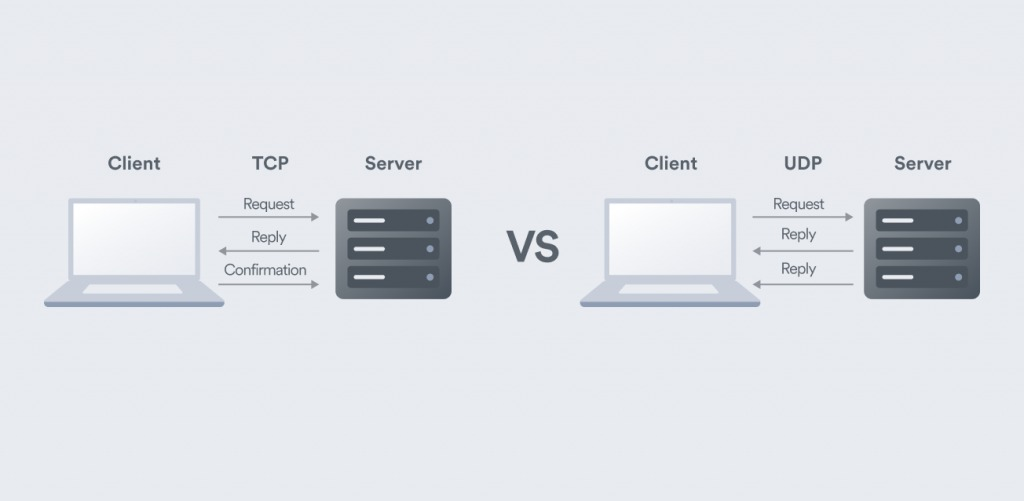
\includegraphics[width=0.7\linewidth]{img/openvpn2.jpeg}
        \caption{OpenVPN hỗ trợ cho TCP và UDP}
        \end{figure}
    \end{itemize} 
\newpage
\subsection*{2.5.4 Nhược điểm của OpenVPN}
 \addcontentsline{toc}{subsection}{2.5.4 Nhược điểm của OpenVPN} 

\begin{itemize}
        \item \textit{Tốc độ chậm hơn:}
        
         Do sử dụng các thuật toán mã hóa mạnh mẽ và cơ chế bảo mật tiên tiến, OpenVPN thường tiêu tốn nhiều tài nguyên hệ thống hơn so với các giao thức VPN khác như PPTP hoặc IKEv2. Việc xử lý mã hóa và giải mã dữ liệu làm giảm tốc độ kết nối, đặc biệt khi sử dụng trên các thiết bị có cấu hình thấp hoặc mạng có băng thông hạn chế.
        \item \textit{Cài đặt thủ công:}

       So với các giao thức khác như PPTP hoặc L2TP, việc cấu hình OpenVPN phức tạp hơn, đặc biệt khi sử dụng chứng chỉ SSL/TLS. Không giống như một số giao thức khác được tích hợp sẵn trên các hệ điều hành hoặc thiết bị mạng, OpenVPN yêu cầu cài đặt phần mềm riêng, gây khó khăn cho người dùng không am hiểu công nghệ.

       
        \item \textit{Có thể yêu cầu ứng dụng bên thứ 3:}

        Không giống như các giao thức VPN được tích hợp sẵn trên nhiều hệ điều hành như L2TP, IKEv2. OpenVPN thường yêu cầu người dùng tải và cài đặt ứng dụng bên thứ ba, chẳng hạn như \textit{OpenVPN Connect}. Điều này có thể gây bất tiện, đặc biệt trong các môi trường hạn chế hoặc không hỗ trợ cài đặt phần mềm bên ngoài. Hơn nữa, việc duy trì và cập nhật ứng dụng cũng cần được quản lý để đảm bảo bảo mật.
    \end{itemize} 

 \section*{2.6 Tổng kế các giao thức của VPN}
 \addcontentsline{toc}{section}{2.6 Tổng kết các giao thức VPN}

 Tóm lại, việc lựa chọn giao thức VPN phụ thuộc vào mục tiêu sử dụng của từng doanh nghiệp, cá nhân. Dưới đây là bảng so sánh tốc độ, bảo mật, độ tương thích, khả năng vượt tường lửa, độ phức tạp khi cấu hình của các giao thức. \newpage

 \begin{table}[h!]
    \centering
    \begin{tabular}{|p{1.5cm}|p{2cm}|p{2.5cm}|p{2.5cm}|p{2.5cm}|p{2.5cm}|}
    \hline
    \textbf{Giao thức}  & \textbf{Tốc độ}  & \textbf{Bảo mật}  & \textbf{Tương thích} & \textbf{Khả năng vượt tường lửa} & \textbf{Độ phức tạp khi cài đặt} \\\hline
    PPTP               & Rất nhanh       &Thấp            & Cao (hầu hết thiết bị)          & Kém                            & Dễ                        \\\hline
    L2TP/ IPsec         & Trung bình      & Cao (nhờ IPsec) & Cao                            & Kém                            & Trung bình                \\\hline
    SSTP               & Nhanh           & Rất cao do có sử dụng SSL/ TLS & Hạn chế (tốt trên Windows)     & Tốt                            & Dễ                       \\\hline
    IKEv2       & Nhanh           & Rất cao        & Trung bình (iOS, macOS, Windows) & Trung bình                    & Trung bình                \\\hline
    OpenVPN            & Trung bình      & Rất cao do có sử dụng OpenSSL & Cao (đa nền tảng)              & Rất tốt                        & Khó        
    \\\hline
    \end{tabular}
    \caption{So sánh các giao thức VPN}
    \label{tab:VPNComparison}
\end{table}

Từ bảng trên có thể thấy rằng mỗi giao thức đều có đặc điểm riêng phù hợp với những nhu cầu khác nhau. 

- PPTP là giao thức có tốc độ nhanh và dễ triển khai nhưng lại có mức độ bảo mật thấp, phù hợp cho các môi trường không yêu cầu cao về an ninh. 

- L2TP/IPsec cung cấp mức độ bảo mật cao hơn nhờ sử dụng IPsec để mã hóa, tuy nhiên hiệu năng bị ảnh hưởng bởi việc mã hóa kép và dễ bị chặn bởi tường lửa. 

- SSTP, với bảo mật mạnh mẽ thông qua SSL/TLS và khả năng vượt tường lửa tốt, là lựa chọn lý tưởng cho người dùng Windows nhưng hạn chế ở mức độ tương thích. 

- IKEv2/IPsec nổi bật với hiệu suất cao, ổn định, đặc biệt hiệu quả trên các mạng di động, nhưng cài đặt có thể phức tạp hơn. 

- Cuối cùng, OpenVPN là giao thức linh hoạt và bảo mật tốt nhất, có khả năng vượt tường lửa mạnh mẽ và tương thích trên nhiều nền tảng, nhưng yêu cầu cấu hình phức tạp hơn so với các giao thức khác. 

Lựa chọn giao thức VPN tối ưu sẽ phụ thuộc vào sự cân đối giữa tốc độ, bảo mật, khả năng tương thích và yêu cầu sử dụng cụ thể.